% !TeX spellcheck = en_US
\documentclass[a4paper, 11pt]{article}
\usepackage{layouts} % Feel free to remove this one
\usepackage{amsmath,amsthm,amssymb}
\usepackage[backend=biber, sortcites, citestyle=numeric]{biblatex}
\usepackage[tt=false]{libertine}
\usepackage{libertinust1math}
\usepackage[T1]{fontenc}
\usepackage{enumitem}
\usepackage[top=1in, bottom=1in, left=1.6in, right=1.6in]{geometry}
\usepackage{graphicx} % Required for inserting images
\usepackage{ifthen}
\usepackage{listings}
\usepackage{siunitx-v2}
\usepackage{subcaption}
\usepackage[most]{tcolorbox}
\usepackage{xcolor}
\usepackage{tikz}

\usepackage[colorlinks, linkcolor=black]{hyperref}

\addbibresource{references.bib}

\numberwithin{equation}{section}

\DeclareCaptionFormat{custom}
{%
	{\sf\footnotesize\textbf{#1#2}{#3}}
}
\captionsetup{format=custom}

% Margin paragraphs
\let\oldmarginpar\marginpar
\setlength\marginparwidth{3cm}
\renewcommand{\marginpar}[1]{\oldmarginpar{\flushleft\tiny\sf{#1}}}

% Colors
\definecolor{primary}{HTML}{5080da}
\definecolor{secondary}{HTML}{da8050}

% tikz definitions
\tikzset{leaf node/.style = {rectangle, draw=black, minimum width = 0.5cm, minimum height = 0.5cm}}
\tikzset{internal node/.style = {circle, draw=black, minimum width = 0.5cm}}

% Theorems
\newtcbtheorem{definition}{Definition}{colback=primary!5, colframe=primary, fonttitle=\bfseries}{def}
\newtcbtheorem{alert}{Alert}{colback=secondary!5, colframe=secondary, fonttitle=\bfseries}{alert}

\theoremstyle{definition}
\newtheorem{exercise}{Exercise}[section]

% Code listings

\definecolor{codegreen}{rgb}{0,0.6,0}
\definecolor{codegray}{rgb}{0.5,0.5,0.5}
\definecolor{codepurple}{rgb}{0.58,0,0.82}
\definecolor{backcolour}{rgb}{0.95,0.95,0.92}

\lstdefinestyle{mystyle}{
	backgroundcolor=\color{backcolour},   
	commentstyle=\color{codegreen},
	keywordstyle=\color{magenta},
	numberstyle=\tiny\color{codegray},
	stringstyle=\color{codepurple},
	basicstyle=\ttfamily\footnotesize,
	breakatwhitespace=false,         
	breaklines=true,                 
	captionpos=b,                    
	keepspaces=true,                 
	numbers=left,                    
	numbersep=5pt,                  
	showspaces=false,                
	showstringspaces=false,
	showtabs=false,                  
	tabsize=2
}

\lstset{style=mystyle}

% Custom commands
\newcommand{\Z}{\mathbb{Z}}
\newcommand{\hint}{\textit{Hint:}~}
\newcommand{\inlcd}[1]{\lstinline[language=Python]{#1}}

% inline code blocks
\newcommand\mystrut{\rule[-1pt]{0pt}{.8em}}

\newtcbox{\code}{on line, boxrule=0pt, boxsep=0pt, top=2pt,
	left=2pt, bottom=2pt, right=2pt, colback=gray!25, colframe=white,
	fontupper={\ttfamily\mystrut}}

% Colors
\definecolor{primary}{HTML}{5080da}

% Theorems
\newtcbtheorem{task}{Task}{colback=primary!5,colframe=primary,fonttitle=\bfseries}{task}

% Custom commands
\newcommand{\player}{\texttt{p}}
\newcommand{\fow}{\texttt{*}}

%%% Local macros
\newcommand{\caret}{\,^\wedge\,}

\title{Programming Lab 01: Creating a Simple Game Environment}
\author{V. Markos\\Mediterranean College}
\date{\today}

\begin{document}
	%
	\maketitle
	%
	\begin{abstract}
		What is this? Probably an ongoing lab for this course, where you will create simple game in Python. Do not expect spectacular graphics and all that stuff, since this course is not about that, but expect to encounter and attack several data structures and algorithm--related problems as we go into more sophisticate designs for our game. Stay tuned for more\ldots
	\end{abstract}
	%
	%
	%
	\section{Introduction (Or Some First Comments)}
	%
	Before we actually start with this lab series, some rough comments on what to expect (and what not to) from this lab:
	\begin{itemize}
		\item This is \textbf{not an introduction to games design.}
		\item This is, and should be treated as such, \textbf{an introduction to Python programming} and, especially, getting our hands dirty with some actual code, other than converting temperatures, checking primality and all that stuff we see in lab exercises.
		\item I do not have a full idea of the final version of the game, yet. And, probably, I will not have until Week 12. Many of the features will be decided on the spot, by you and me, as we discuss in class.
		\item However, I do have a plan on what this game will assess, in terms of data structures and relevant algorithms. Consequently, there are certain features that I have already decided to include.
		\item However (vol.~2), I also have a certain rough plan for the abstract game outline. There will be a simple game grid, initially covered by a Fog of War, and you will have a player exploring the grid while having to avoid computer--controlled enemies and find some relics which will be collectible and stuff like that --- we will further specify features together throughout the next weeks.
	\end{itemize}
	%
	%
	%
	\section{Designing A Game Grid}
	%
	As a first step, we shall start by designing a game grid. So, since the grid is initially covered by the Fog of War, we will just print a $20\times 20$ grid full of asterisks, as the one shown in Figure~\ref{fig:game grid}. So, here comes your first task:
	
	\begin{task}{Printing the Game Grid}{task01}
		Write a python function that prints a $20\times 20$ grid as the one shown in Figure~\ref{fig:game grid}.
	\end{task}
	
	\begin{figure}[tb]
		\centering
		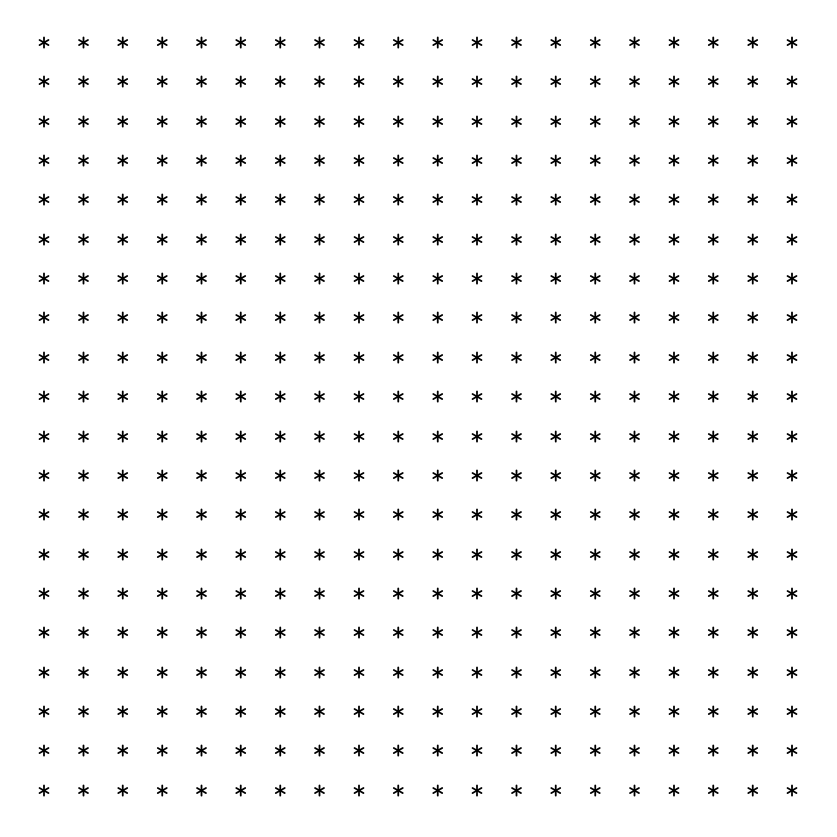
\begin{tikzpicture}
			\foreach \i in {1,...,20} {
				\pgfmathsetmacro{\xcoord}{0.5*\i}
				\foreach \j in {1,...,20} {
					\pgfmathsetmacro{\ycoord}{0.5*\j}
					\node (\i\j) at (\xcoord, \ycoord) {\fow};
				}
			}
		\end{tikzpicture}
		\caption{Our initial $20\times 20$ game grid, covered by the Fog of War\ldots}
		\label{fig:game grid}
	\end{figure}
	
	Now, what if we want in the future to allow players choose the size of the game grid? For instance, some players might want to play a quick round of our (nameless) game while some others might want to spend some time on it. It would be nice to have some predetermined grid sizes to allow the players choose from. Let's say we offer three options:
	\begin{itemize}
		\item A small, $15\times 15$, grid;
		\item A medium sized, $20\times 20$, grid, and;
		\item A large, $30\times 30$, grid.
	\end{itemize}
	
	Here comes your next task:
	\begin{task}{Customisable Game Grids}{task02}
		Improve your previous version of the grid printing function to accommodate the above three sizes. You should ask the user for their preference (making sure the user provides a valid input), and draw the corresponding grid on screen. You can also allow for a default option, if you want to (to this end, Python's default values for function arguments might come in handy).
	\end{task}
	%
	%
	%
	\section{Creating a Player}
	%
	So far, we have implemented a simple grid printing function and provided the user with the option to choose level size. But, no player has appeared on the grid so far. So, to begin with, we should make a player show up on the grid, as shown in Figure~\ref{fig:player on grid}.
	
	\begin{task}{Printing the Main Character}{task03}
		Print the game's main character (which will be controlled by the player themselves) on the game grid. The character's starting position should be at the bottom left corner of the grid, as shown in Figure~\ref{fig:player on grid}. The player position should be denoted by the lowercase letter \texttt{p}.
	\end{task}
	
	\begin{figure}[tb]
		\centering
		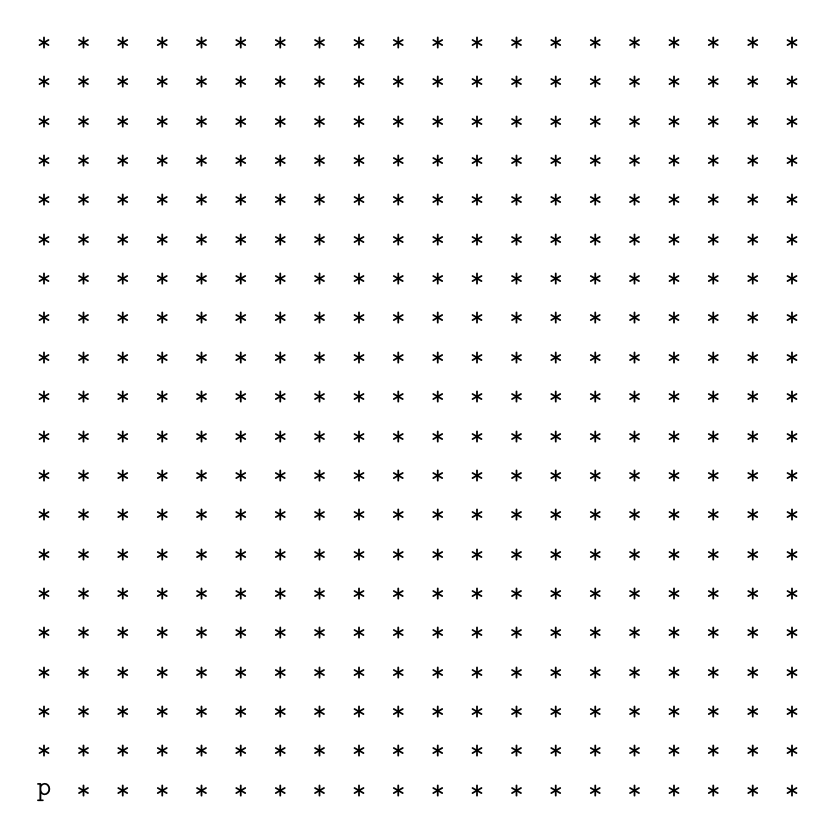
\begin{tikzpicture}
			\foreach \i in {1,...,20} {
				\pgfmathsetmacro{\xcoord}{0.5*\i}
				\foreach \j in {1,...,20} {
					\pgfmathsetmacro{\ycoord}{0.5*\j}
					\ifthenelse{\i=1\AND\j=1}{
						\node (\i\j) at (\xcoord, \ycoord) {\player};
					}{
						\node (\i\j) at (\xcoord, \ycoord) {\fow};
					}
				}
			}
		\end{tikzpicture}
		\caption{A $20\times20$ grid with our game's main character printed at the bottom left position of the grid (denoted by a \player).}
		\label{fig:player on grid}
	\end{figure}
	
	We have a grid, we have a (visible) main character, what is still missing? \textbf{Movement!} We should allow our player to move the main character around so long as they stay within the game's grids. We will allow four types of movement:
	\begin{itemize}
		\item North, i.e., upwards, which will be implemented whenever the player enters the character \texttt{n}.
		\item South, i.e., downwards, which will be implemented whenever the player enters the character \texttt{s}.
		\item West, i.e., leftwards, which will be implemented whenever the player enters the character \texttt{w}.
		\item East, i.e., rightwards, which will be implemented whenever the player enters the character \texttt{e}.
	\end{itemize}
	In all cases, the main character should move by \textbf{one cell}. These are the only possible moves that are allowed, so here comes your next task:
	
	\begin{task}{Moving Around}{task04}
		Implement character movement as described above. You should take into account the following:
		\begin{itemize}
			\item No other form of movement, e.g., diagonally or skipping cells is allowed.
			\item You should properly check for and prohibit movement outside the grid's boundaries. In such cases, the user should be informed by an appropriate message and a new instruction should be asked for.
			\item You are free to choose whether you will accept both lowercase (\texttt{nswe}) and / or uppercase (\texttt{NSWE}) movement instructions.
		\end{itemize}
		In the above, you should take into account how you will properly store the main character's location, i.e., which Python data structure is the most appropriate for that purpose? Also, how are you going to implement the game loop?
	\end{task}
	%
	%
	%
	\section{Further Considerations}
	%
	So far, we have implemented some simple yet fully functional (hopefully) game mechanics. What follows below is not necessary to be implemented for the next labs, but serves more as some further thoughts that could help you work on some interesting problems. Here are two simple tasks to get you started:
	\begin{task}{Circular Movement (Grid Wrapping)}{task05}
		In Task~\ref{task:task04} we prohibited movement beyond the grid boundaries. However, this is not the only way to handle boundaries in our game. Another option could be to allow the player move from one side of the grid to the other, i.e., west from the westmost end of the grid would make the main character appear on the same row, just at its eastmost part, moving south from the southmost part of the grid would result to the main character appearing on the same column, just on the southmost part and so on.
		
		Bearing in mind the above, implement the above circular movement across the game board. Which one do you prefer as the default way? If you want to, you can allow players to choose how their character will move around the grid, i.e., whether movement will be restricted, as implemented in Task~\ref{task:task04} or unrestricted as here.
	\end{task}
	
	Playing around and testing our game so far, you might have observed that re--printing the grid every time is a bit cumbersome and also results to a really stacked output on the terminal. You next task requires you to devise ways to avoid printing the grid all the time.
	
	\begin{task}{Overwriting the Game Grid}{task06}
		Using special ASCII / Unicode characters, and especially the carriage return character, \texttt{\textbackslash r}, improve the grid printing function so that each time the main character moves, the grid is not printed below the previous version of the grid but on top of it, essentially saving up space on the terminal's feed.
	\end{task}
	%
	%
	%
\end{document}
